\begin{par}
    \par \hspace{15pt} Although the field of music generation is not as well developed as the field of image generation, there are still some rather impressive works that can generate drum beats or music in general. The model that the group is most interested in is the MuseGAN \cite{musegan} model. It is a multi-track sequential generative adversarial network. It the state-of-the-art temporal model at its time for symbolic music generation, and is one of the only known models for generating polyphonic music. 

    \begin{figure}[H]
        \centering
        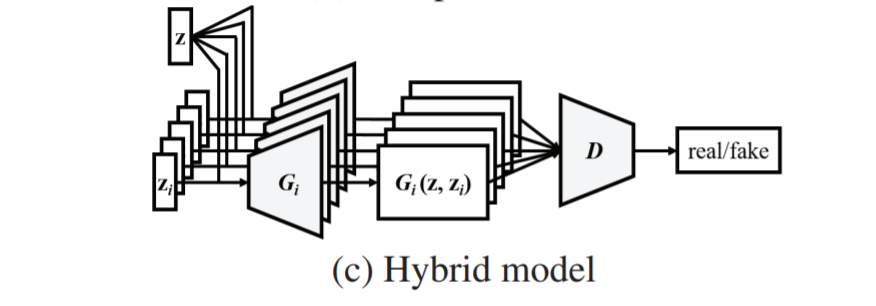
\includegraphics[width=3in]{image/hybrid_model}
        \caption{MuseGAN: Hybrid model}
        \label{fig:hybrid}
    \end{figure}

    \par \hspace{15pt} In this course project, we are expecting to utilize the Hybrid model in Figure \ref{fig:hybrid} from MuseGAN. In this architecture, each segment GAN has one local Gaussian random vector input $z_i$ and a global Gaussian random vector input $z$. $z_i$'s are most likely different for each segment generator, and $z$ would remain the same for each segment generators, serving as an artificial inductive bias for all generator to produce more style-aligned music for a single song. Then the GAN is expected to generate a segment of track using these two random vectors. 

    \par \hspace{15pt} However, the goal of the MuseGAN model diverges from this course project, since it focuses on generating all tracks from scratch using a relatively large-scale Generative Adversarial Network (GAN). In this course project, the main focus was to generate drum tracks from other instruments by using a lighter model. To adapt this objective, the team would first like to perform a classification/encoding task on the existing tracks from other instruments, and serve this encoded vector as the inductive bias to further facilitate each segment GAN. Moreover, the team is also expecting to explore different loss implementation and discriminator architectures to further simplify the model while remaining the same performance. 

    
    % \par This paper has suggested that the convolutional neural networks (CNN) could offer optimal performance in recognizing local, translation-invariant patterns. Such observation was also confirmed in an internet article \cite{lamb_of_God} that discussed generation of drum beats for non-drum musics. It was specifically addressed that CNN could usually out-perform LSTM while longer input length is offered during training. Beyond that, training the CNN models would be more attainable for this course project comparing to the computation equipment needed for training LSTM models.

    % \par Another important implementation details about the MuseGAN is the way this model uses to segment the input music into fixed size matrices for CNNs, namely the multi-track piano-roll representation. This representation has made possible for this course project to fine tune some GAN or CNN with different architecture and compare their performance against the existing models. 

    % However, the focus of this paper was rather broad comparing to the scope of this project, due to its polyphonic generation nature. It also incorporates RNNs, namely Long Short-Term Memory Networks (LSTM). This course project, on the other hand, would focus more on a single-track generation model that is easier to train. However, the main ideas of this project were largely based on the MuseGAN model, which would be discussed in further details in Section \ref{sec:approach}.
    
    % \par There are also many successful models that concentrates only on generating drum beats under different conditions. 
    % \textbf{INCOMPLETE}

    % \par However, the models mentioned above are all Recurrent Neural Network (RNN) paired with a Discriminator. RNN are known for their difficulties in training. They require tremendous amount of computation resources, and usually takes a lot of time for training before the result of the model becomes acceptable. For a course project, the group would have neither the computation power nor the time, so the group would like to investigate how well light-weight models, or even supervised learning model would perform in the music generation tasks. 

\end{par}